\documentclass[titlepage, 11pt, a4paper]{article}
\usepackage[utf8]{inputenc}
\setlength{\parindent}{20pt}
\linespread{1.25}
\usepackage{csquotes}
\usepackage{etoolbox}
\usepackage[round, sort, comma]{natbib}
\setlength{\bibsep}{1pt}
\usepackage[dvipsnames]{xcolor}
\apptocmd{\thebibliography}{\renewcommand{\sc}{}}{}{}
\usepackage[colorlinks=true,linkcolor=Blue, citecolor=Blue]{hyperref}
\usepackage{titlesec}
\newcommand{\headingfont}{}
\titleformat*{\subsection}{\headingfont\bfseries\small}
\titleformat*{\subsubsection}{\headingfont\bfseries\small}
\usepackage{amsmath, amssymb}
\usepackage[ceqn]{nccmath}
\usepackage[toc,title,page]{appendix}
\renewcommand{\&}{and}
\usepackage{geometry}
\geometry{left=3cm, right=3cm, top=1.5in, bottom=1.5in}
\frenchspacing
\usepackage{booktabs}
\usepackage{graphicx,wrapfig}
\usepackage{multirow}
\usepackage{float}
\usepackage{titling}
\PassOptionsToPackage{svgnames}{xcolor}
\usepackage{tcolorbox}
\tcbuselibrary{skins,breakable}
\usetikzlibrary{shadings,shadows}
\usepackage[colorinlistoftodos,prependcaption,textsize=small]{todonotes}
\usepackage{siunitx}
\sisetup{round-mode=places, round-precision=3, detect-all}



\begin{document}


\thispagestyle{empty}
\begin{center}
    \vspace*{2cm}

    {\Large \bfseries Public investment and supply \par}
    \vspace{1.5cm}

    {\large
    Paula Bejarano Carbó \footnote{National Institute of Economic and Social Research and University of Oxford} \quad
   Benjamin Caswell \footnote{National Institute of Economic and Social Research} \quad Stephen Millard\footnote{National Institute of Economic and Social Research, Durham University Business School, Portsmouth University and Centre for Macroeconomics} \par }

   
    {\large \today \par}
    \vfill
   

    \begin{minipage}{0.9\textwidth}
    \textbf{Abstract} \\
    \noindent
    In this paper, we investigate the link between public investment and output in the United Kingdom. We estimate a medium-scale neoclassical growth model in order to gauge the output elasticity of public capital for the UK economy, finding a posterior mean of 0.112 for the elasticity, indicating that public capital has a positive and economically meaningful effect on output in the UK.  
    Using the results from the estimation exercise, we find that the welfare-maximising output share of public investment is between 5.9  and 6.1 per cent, above the historical average of around 3.5 per cent. 
    This finding, though interpretable as a reasonable upper bound, suggests that the United Kingdom has scope to benefit from an increase in productive public investment.
    Our results suggest that further work in estimation of the output elasticity of public capital may be the most fruitful avenue for future research.
    \end{minipage}

    \vfill
\end{center}
\newpage
% --- End manual title page ---

\tableofcontents 
\thispagestyle{empty}

\pagebreak 

\setcounter{page}{1} 
\section{Introduction}
In this paper, we investigate the link between public investment and output in the United Kingdom. As is well known, productivity growth – as measured by output per hour worked – has been stagnant, particularly in the aftermath of the Global Financial Crisis. 
While there are many contributors to this, standard economic growth accounting indicates that this is driven by declining growth in total factor productivity (TFP) and capital accumulation \citep{chadha2025understanding}. 
As argued by Chadha and Samiri, the latter capital shallowing trend is particularly puzzling as it has occurred alongside cheap financing costs. 

At the same time, the United Kingdom's public investment to GDP ratio has been low by historical and international standards since the late 1970s. Fiscal stimulus is well-known to have demand-side effects in the short run. An increase in public investment spending in infrastructure, for example, will instantly raise demand for labour and capital inputs. 
In contrast to government consumption spending, \textit{productive} public investment spending can also have supply-side effects in the medium and long run. For example, the same increase in infrastructure spending may unlock further private investment by increasing the return to private capital and labour inputs. This is especially relevant when such spending has public good characteristics - as the market underprovides goods where the marginal social benefit exceeds the marginal private benefit.

Over time, this additional business investment may expand an economy's production potential beyond the initial increase in public capital. 
Following this logic, it is certainly possible that low public investment in the United Kingdom could be, at least, part of the explanation of low UK productivity growth.
However, the extent to which each additional pound spent on this productive public capital will boost economic output - the public investment multiplier - is an open question. As noted, public capital spending interacts with the wider economy; a cost-benefit analysis of individual projects aggregated-up is likely to underestimate the returns to public investment. A quantitative analysis that evaluates the full costs and benefits of public investment, inclusive of general equilibrium effects, is therefore crucial to informed fiscal policymaking. 

Methodological challenges complicate investigating the link between public investment and output. Most notably, any modeling conclusions reached will be particularly sensitive to the calibration of the output elasticity of public capital. As is detailed in section (\ref{section2}) below, estimating this parameter empirically is challenging, and there is limited  UK-specific evidence. 
Additionally, public investment simultaneously operates as a short-run demand stimulus and as an input into medium- to long-run productive capacity.  These distinct channels operate over different horizons and are typically analysed using different modeling frameworks, creating a methodological tension when attempting to study both within a unified empirical or theoretical setting.


To investigate this matter given the above challenges, we build a medium-scale neoclassical growth model where we allow increases in public investment to affect the marginal productivity of labour and private capital, thus creating a mechanism through which public investment can affect aggregate supply as well as aggregate demand. We then estimate this model via Bayesian techniques, feeding in UK-specific data to obtain values for key parameters, in particular, the elasticity of output with respect to public capital. This approach helps us circumvent many of the challenges that empirical approaches to estimating this elasticity face.
We then use our estimated model to estimate the welfare-maximising share of public investment in output, in order to gauge where the United Kingdom's public investment to GDP ratio has been relative to the model-implied optimum.

Although much work has been done looking at the effects of public-sector investment, particularly in infrastructure and military spending, this remains a relatively under-researched area in the United Kingdom. This paper therefore aims to provide a quantitative analysis of the link between public investment and output in the United Kingdom, with a particular focus on estimating the output elasticity of public capital.
Our results provide a quantitative contribution that can complement the wider literature and can help inform current fiscal policymaking in the United Kingdom, as well as provide a framework for questions surrounding role of public investment in shaping the United Kingdom's productivity growth.  

The rest of the paper is organised as follows: section (\ref{section2}) presents the related literature; section (\ref{section3}) outlines our baseline theoretical model to build intuition; section (\ref{estimation}) estimates this model while section (\ref{simulation}) quantifies the effects of a simulated rise in public investment in the United Kingdom; section (\ref{conclusion}) concludes.


\section{Related literature} \label{section2}
This paper relates to work evaluating the macroeconomic effects of government investment - which can best be divided into an empirical and a theoretical literature. 

\subsection{Empirical literature} \label{lit1}
There is a wide empirical literature focused on estimating the relationship between government spending and output - often referred to as the fiscal multiplier - in advanced economies (see, e.g., Blanchard and Perotti (\citeyear{blanchard2002empirical}); Coenen et al. (\citeyear{coenen2012effects}); Bayer et al. (\citeyear{bayer2023coronavirus}); Sousa (\citeyear{sousa2025taking})). Two important sub-strands of this field are ones which seek  to estimate the state-dependency of the fiscal multiplier (see, e.g., Auerbach and Gorodinchenko, (\citeyear{auerbach2012measuring}); Ramey and Zubairy (\citeyear{ramey2018government})), and separately, narrow their focus to the consequences of military spending on output (see, e.g., Ramey and Shapiro (\citeyear{ramey1998costly}); Sousa (\citeyear{sousa2025taking})). The literature that best speaks to this paper, which specifically analyses the effect of
public investment on aggregate output in advanced economies, is considerably narrower. For some reviews of this literature, see, e.g., Romp and den Haan (\citeyear{romp2007public}) and Pereira and Andraz (\citeyear{pereira2013economic}). 

Studies estimating the output elasticity of public capital are best divided by methodology. The ‘production function approach’ assumes that public capital enters the aggregate production function either directly, or as a determinant of total factor productivity, and estimates this equation using aggregate data  
(see, e.g., Bom and Ligthart (\citeyear{bom2014have}); Heintz (\citeyear{heintz2010impact})).  Panel data methods applied to the production function approach include, e.g. Arslanalp et al. (\citeyear{arslanalp2010public}). A smaller literature employs the `cost function approach' which aims to quantify the effect of public investment on private firms' costs (see, e.g.: Nadiri and Mamuneas (\citeyear{nadiri1991effects}); Demetriades and Mamuneas (\citeyear{demetriades2000intertemporal})). 
These approaches have drawn methodological critique mainly due to concerns around endogeneity (changes to public capital are often endogenous to the state of the economy or to firm needs) and around model mis-specification (due to needing to assume rigid functional forms). More concerningly, these approaches yield an extremely wide array of estimates of the output elasticity of public capital (ranging from -1.7 to 2.04 in Bom and Ligthart's (\citeyear{bom2014have}) meta-analysis of 68 papers), rendering it incredibly challenging to draw conclusions from them.


Vector autoregression modeling approaches include, e.g., Kamps (\citeyear{kamps2005dynamic}) and de Jong et al. (\citeyear{de2017effect}). While VARs can overcome the concerns around mis-specification in the above approaches, it remains challenging to draw conclusions from this literature for the purposes of this paper due to mixed evidence on the sign of the public investment multiplier.
Recent papers have estimated the causal effects of public investment by employing a local projections approach (see, e.g., Abiad et al. (\citeyear{adb2016macroeconomic}); Deleidi et al. (\citeyear{deleidi2020public})), finding positive short and medium-run multipliers.
While it is promising to have some consensus around the sign of these multipliers, neither paper provides an estimate of the output elasticity of public capital for the United Kingdom. 
A key challenge of replicating this approach is that it requires identification of exogenous and unanticipated public investment shocks.

As noted, it is difficult to draw conclusions from the empirical literature on the output elasticity of public capital in the UK due to the compounding issues of evidence being highly mixed, and not UK-specific. The few papers that we are aware of that report UK-specific estimates reach diverging conclusions that are representative of the wider state of the literature: for example, Demetriades and Mamuneas (\citeyear{demetriades2000intertemporal}) use the cost function approach to estimate a long and short-run output elasticity of 0.36, while Kamps (\citeyear{kamps2005dynamic})'s seminal VAR paper reports a negative short-run elasticity and a long-run elasticity of 0.08 - though the latter is not statistically significant. In Bom and Ligthart's (\citeyear{bom2014have}) meta-analysis of 68 papers, they report only one study which offers UK-specific estimates, compared to 31 studies for US-specific estimates. In their meta-regression of the output elasticity of public capital, they find the country dummy for the UK to be negative - though this result is not statistically significant.

 

We leave addressing this gap for future research, and instead rely on this literature when forming our prior beliefs in the estimation of our DSGE model.


\subsection{Theoretical modeling}
Much of the work on theoretical modeling of government investment spending can be traced back to Baxter and King (\citeyear{baxter1993fiscal}), which incorporates government consumption and government investment spending in an Real Business Cycle (RBC) model to show that a permanent increase in public spending can generate output multipliers that exceed 1. In the baseline Baxter and King model, government consumption and investment spending enter the resource constraint in the same way – implying that a government that increases its spending extracts resources from the economy – and thus an increase in either comes at the cost of a negative wealth effect (households decreasing consumption and raising labour supply) in the short run.
At the same time, an increase in government investment transmits directly to the supply side via the production function, which includes public capital as a factor of production. In the medium-run, this increase also boosts output indirectly by raising the marginal products of capital and labour, incentivising firms to invest in private capital and demand more labour. Through this additional mechanism, an increase in government investment has larger effects on output and private investment than unproductive government consumption spending in the medium and long term. 

Several papers have since extended the Baxter-King framework within the RBC setting (see, e.g., Ramey and Shapiro (\citeyear{ramey1998costly}); Burnside et al. (\citeyear{burnside2004fiscal})) as well as the New Keynesian setting (see, e.g. Coenen et al. (\citeyear{coenen2012effects}); Boehm (\citeyear{boehm2020government}); Ramey (\citeyear{ramey2020macroeconomic}); Ganelli and Tervala (\citeyear{ganelli2020welfare}); Tervala and Watson (\citeyear{tervala2022hysteresis})).

%There is also a wide literature examining fiscal policy in New Keynesian models. Notable papers from this wide literature include, for example: Galí et al. (\citeyear{gali2007understanding}), Christiano et al. (\citeyear{christiano2011government}), Eggertsson (\citeyear{eggertsson2011fiscal}) and Jo and Zubairy (\citeyear{jo2025state}). The literature extending the Baxter and King framework in a New Keynesian setting to focus on the macroeconomic effects of government investment spending specifically is narrower. Coenen et al. (\citeyear{coenen2012effects}) include a CES-aggregate of private and public capital within an aggregate Cobb-Douglas production function to estimate an extended version of the ECB's New Area-Wide Model, finding a high long-run output elasticity of public investment due to high complementarity between public and private capital. On the other hand, Boehm (\citeyear{boehm2020government}) builds a two-sector model with imperfect factor mobility, finding that the output multiplier for government investment is significantly smaller than the multiplier for government consumption. 

%Notable papers from this wide literature include: Galí et al. (\citeyear{gali2007understanding}), who introduce hand-to-mouth consumers in a two-agent model to reconcile the empirically observed fact that an increase in government consumption spending leads to an increase in private consumption; Christiano et al. (\citeyear{christiano2011government}) and Eggertsson (\citeyear{eggertsson2011fiscal}), who provide evidence that fiscal multipliers can be larger when interest rates are their zero lower bound; and Jo and Zubairy (\citeyear{jo2025state}), who introduce a downward nominal wage rigidity to analyse the state-dependency of the fiscal multiplier more broadly. More recently, a small literature has considered the effects of government spending in search-and-matching environments to understand the interaction between government spending and spare capacity in goods markets (see, e.g., Ghassibe and Zanetti (\citeyear{ghassibe2022state})).





This paper is most similar to work featuring estimated extensions of the Baxter-King model. Leeper et al. (\citeyear{leeper2010government}) estimate a medium-scale extension of Baxter-King and focus their analysis on the effects of time-to-build delays in the formation of public capital. The authors conduct policy scenarios considering different values of the output elasticity of capital as well as different lengths of the public investment implementation delays. Conditional on fixing this elasticity to 0.1, the authors estimate a cumulative public investment multiplier of between 0.9 and 1.14; these figures drop to 0.31 and 0.39 for an elasticity of 0.05. Sims and Wolff (\citeyear{sims2018output}) consider an estimated medium-scale New Keynesian extension of the Baxter-King model, but this paper also relies on fixing the elasticity of output to public capital at 0.05. The authors find that, conditional on this elasticity, the optimal public investment to GDP ratio is 0.057 in steady state. 


Our paper is most similar to Ercolani and Valle e Azevedo (\citeyear{ercolani2014effects}). Similarly to Leeper et al. (\citeyear{leeper2010government}), this paper estimates a medium-scale Baxter-King style RBC model for the United States, but makes a further contribution in that they are able to directly estimate the output elasticity of public capital and provide evidence that this parameter is locally identified. However, when using their preferred specification of an uninformative prior, the authors find that the posterior mode of the output elasticity of public capital in the United States is zero. 

Another highly relevant paper is the recent OBR report which investigates the role of public investment and potential output in the United Kingdom \citep{Suresh24}. In this paper, the authors simulate a 1 per cent of GDP increase in public investment in a partial equilibrium framework, finding that when they calibrate the output elasticity of public capital to 0.1, long-run output increases by 2.4 per cent. 
While this paper makes an important first step in applying accounting frameworks from the literature to the UK context, we find that the additional insights provided by a DSGE model are essential in exploring this complex policy issue.

Our paper thus complements this public investment literature by building and estimating a quantitatively relevant DSGE model for the United Kingdom. Through this, we are able to estimate the elasticity of output to public capital through Bayesian techniques, allowing us to conduct policy-relevant simulations of the UK economy. 



\section{Neoclassical model} \label{section3}

As noted in the introduction, investigating the link between public investment and economic growth is challenging from a modeling perspective for two main reasons. Firstly, results will be particularly sensitive to the output elasticity of public investment chosen (and, as noted in the literature review, there is limited evidence on the value for this parameter in the UK context). Secondly, there is a potential tension in terms of modeling choice due to the fact that public investment simultaneously operates as a short-run demand stimulus and as an input into medium- to long-run productive capacity. 

We find that the best approach to tackle these challenges is to build and estimate a medium-scale extension of the Baxter-King RBC model.
In particular, obtaining an estimate for our key parameter of interest - the elasticity of output to public capital - via Bayesian techniques allows us to circumvent many of the methodological issues that empirical approaches face, described in section (\ref{lit1}).
Additionslly, this approach allows us to draw on more information (importantly, UK-specific data) than a smaller, more parsimonious model would.


This section therefore describes a medium-scale neoclassical model. This description will focus on outlining key departures from the workhorse RBC model. A complete exposition of the model derivation can be found in the appendix. 

\subsection{Key model elements}
The fundamental model dynamics explored in this paper arise from including public capital as a factor in the aggregate Cobb-Douglas production function, as in the canonical Baxter and King (\citeyear{baxter1993fiscal}) model:   


    \begin{equation} \label{agg_prod_fn} 
    Y_t= A_t K_{g,t}^{\theta}\tilde{K}_{p,t}^{\alpha}N_t^{1-\alpha}
\end{equation}
where $Y_t$ is aggregate output, $A_t$ denotes an aggregate productivity shock, 
$K_{g,t}$ denotes the public capital stock, $\theta$ is the elasticity of output to public capital, 
$\tilde{K}_{p,t}$ is the effective private capital stock (allowing for variable private capital utilisation), $\alpha$ is the elasticity of output to private capital, $N_t$ denotes the aggregate labour input, and the elasticity of output to labour is given by $1-\alpha$ where the 1 ensures that the production function exhibits constant returns to scale in private factors. 

Public capital $K_g$ is formed via public investment, $I_g$. We set public investment as a fixed proportion, $s_g$, of GDP: 
\begin{equation}
    I_{g,t} = s_gY_tG^s_{i,t}
\end{equation}
where $G^s_{i,t}$ is an exogenous shock to government investment spending.


We interact this key feature of augmenting the aggregate production function with public capital as a factor of production with additional non-standard frictions and rigidities, namely: investment adjustment costs, variable capacity utilisation, time-to-build delays on public investment, and distortionary taxes. 

\begin{itemize}        
    \item \textbf{Investment adjustment costs on private capital:} \par 
    This friction captures market imperfections and financial constraints which may prevent investment from jumping immediately to its socially optimal level following a shock. This feature is quantitatively important as it reduces the volatility of private investment following a shock, in line with the data. In our model, this cost appears as a quadratic term in the household's capital accumulation constraint: 
    \begin{equation} \label{cap_accum}
         K_{p,t+1} = (1-\underbrace{\delta_{p}U_{k,t}^\phi}_{=\delta_{p,t}})K_{p,t} + I_{p,t}\Big(1-\frac{\kappa}{2}\Big[ \frac{I_{p,t}}{I_{p,t-1}} -1 \Big]^2\Big)X_t
    \end{equation}
    where $I_{p,t}$ is the household's private investment, $\kappa$ governs the size of the adjustment cost, $X_t$ is a shock to the marginal efficiency of investment and $\delta_{p,t}$ is the effective depreciation rate on private capital, explained in the bullet point below.

    \item \textbf{Variable capacity utilisation of private capital:} \par 
    In the workhorse RBC model, private capital services are proportional to the stock of private capital - a feature which we do not observe in the data. Including variable capacity utilisation in this model is quantitatively important as it enables cyclicality in private capital accumulation, as observed. In our model, this friction appears in equation (\ref{cap_accum}) above via the effective depreciation rate on public capital, $\delta_{p,t}$, as well as in the household's budget constraint: 

    \begin{equation} \label{nom_BC}
        C_t(1+\tau_c) + I_{p,t}  = W_tN_t(1-\tau_n) + R_{k,t}(1-\tau_k)U_{k,t}K_{p,t} +D_t  - T_t 
    \end{equation}
    where $C_t$ is private consumption; $\tau_i,  i\in \{c,k,n\}$ represent taxes on consumption, private capital income and labour income, respectively; $W_t$ is the real wage; $D_t$ are firm dividends paid to households; $N_t$ denotes hours worked; $R_{k,t}$ is the real return to private capital; and $T_t$ denotes a lump-sum tax.  
    
    The equations above indicate that the existing stock of private capital can be worked more intensively (via an increase in $U_{k,t}$), but at the cost of accelerated depreciation, where $\phi$ governs the magnitude of that cost. Here, $\delta_p$ represents the baseline rate of physical depreciation and $\delta_{pt} = \delta_{p}U_{k,t}^\phi$ is the effective depreciation rate. When capital is utilised more intensively, the existing stock depreciates more quickly as $\phi > 0$. The product $U_{k,t}K_{p,t} = \tilde{K_{p,t}}$ represents the flow of private capital services. This means that private capital services can adjust immediately in response to a shock, without the firm having to wait one period for investment to roll over into capital stock. Subsequently, it is private capital services which enters as a factor of production in the aggregate production function in equation (\ref{agg_prod_fn}).

    \item \textbf{Time-to-build delays on public investment} \par
    Drawing from Suresh et al. (\citeyear{Suresh24}), we model public investment purchases as facing time-to-build lags, delaying the process through which public investment tranforms into a part of the productive public capital stock, in order to match observed data. Let $\omega_n$ be the fraction of $I_{g,t}$ that becomes effective at time $t+n$. We write the public capital law of motion as: 

\begin{equation}
    \label{public_LOM}
    K_{g,t+1} = (1-\delta_g)K_{g,t} + \sum_{n=0}^{10}(1-\delta_g)^n \omega_n I_{g,t-n}
\end{equation}


    \item \textbf{Distortionary taxes:} \par 
    Equation (\ref{nom_BC}) indicates that households face distortionary taxes on consumption, private capital income and labour income, as is relevant in the UK context. 

    
\end{itemize}



\section{Bayesian estimation of the model} \label{estimation}
In order to obtain the parameter values needed to complete this model, we use a combination of calibration (zero standard deviation prior) and Bayesian estimation. 

\subsection{Parameter calibration} 
We determine several parameters through calibration using UK data from the first quarter of 1971 to the fourth quarter of 2017 available from the ONS\footnote{Precise details of which data series we used, including the relevant ONS codes, available on request.}, summarised in table (\ref{calibrated_params}). 

We set the discount factor to target the average quarterly real risk-free rate; over our sample period, this averaged 4.21 per cent, implying a discount factor, $\beta$, of 0.989. The weight for private consumption relative to government consumption, $\gamma$, is given by equation (\ref{GC}) in the appendix and ensures that the steady-state ratio of government consumption to private consumption in the model matches the average ratio in the UK data over our sample period. We set the elasticity of substitution for goods to 11, implying a steady-state markup of 1.1, in line with Burgess et al. (\citeyear{burgess2013bank}) and Albuquerque et al. (\citeyear{albuquerque2025decompositions}). For the depreciation rates for private and public capital, we use the average values of the series for depreciation rates calculated within NIESR, using ONS data on capital consumption by sector over our sample period\footnote{The relevant series can be found in our NiGEM database, available to NiGEM subscribers. The codes for private- and public-sector capital depreciation rates are UKKBDEP and UKKGDEP, respectively. Details of how these measures are calculated available on request.}. The consumption tax is given by the average rate of Value Added Tax (VAT) in the United Kingdom over our sample period. The tax rates on labour and capital are given by the average effective rates of income and corporation tax over our sample period.   Finally, we set $s_g$ to match the average public investment to GDP ratio over our sample period.\par 

Two parameter values follow from the solution of the analytical steady state of this model. The parameter which governs the extent to which variable capacity utilisation increases the depreciation of private capital, $\phi$, is calibrated to match a normalised steady-state utilisation rate of 1. The disutility weight on labour, $\nu$, targets a normalised steady state labour supply of 1.

\begin{table}[H] 
\centering
\caption{Calibrated Parameters} 
\begin{tabular}{lll}
\toprule
\textbf{Parameter Name} & \textbf{Symbol} & \textbf{Value} \\
\midrule
Subjective Discount Factor & $\beta$ & 0.989 \\
Private Consumption Utility Weight & $\gamma$ & 0.765 \\
Private Capital Depreciation Rate & $\delta_p$ & 0.022 \\
Public Capital Depreciation Rate & $\delta_g$ & 0.017 \\
Goods Elasticity of Substitution & $\epsilon$ & 11 \\
Consumption Tax Rate & $\tau_c$ & 0.157 \\
Capital Tax Rate & $\tau_k$ & 0.231 \\
Labour Tax Rate & $\tau_n$ & 0.219 \\
Public investment to GDP ratio & $s_g$ & 0.035 \\
Effective depreciation rate cost & $\phi$ & 1.467\\
Disutility weight on labour & $\nu$ & 0.523 \\
\bottomrule
 \label{calibrated_params}
\end{tabular}
\end{table}


\par 
Finally, the $\omega_{t+n}$ parameters, which represent the fraction of public investment made at time $t$ that become effective at time $t+n$, follow from \cite{Suresh24}.

\begin{table}[H]
    \centering 
    \caption{Time-to-build weights}
    \begin{tabular}{c|c|c|c|c|c|c|c|c|c|c|c}
    \toprule
       & t & t+1 & t+2 & t+3 & t+4 & t+5 & t+6 & t+7  & t+8 & t+9 & t+10   \\ \toprule
       $\omega$ & 0 & 0.2 & 0.2 & 0.15 & 0.1 & 0.075 & 0.075 & 0.05 & 0.05 & 0.05 & 0.05 \\
    \bottomrule
    \end{tabular}
    \label{tab:my_label}
\end{table}

\subsection{Parameter estimation}
We next proceed to estimating the remaining parameters in the model, inclusive of shock persistence and size. 
We take observable data from the ONS for GDP, business investment, government consumption, government investment, and private consumption. Given that our model has no trend, we HP-filtered each of these series with the smoothing parameter, $\lambda$, set at its usual value of 1,600. 
We introduce four shocks to the model: productivity, marginal efficiency of private investment, government consumption purchases, and government investment spending. These shocks all follow standard AR(1) processes as follows: 

\begin{gather*}
    log(A_t) = \rho_a log(A_{t-1}) + \varepsilon_{a,t} \\ 
    log(X_t) = \rho_x log(X_{t-1}) + \varepsilon_{x,t} \\ 
    log(G^{s}_{c,t}) = \rho_{gc} log(G^s_{c,t-1}) + \varepsilon_{gc,t} \\
    log(G^s_{i,t}) = \rho_{gi} log(G^s_{i,t-1}) + \varepsilon_{gi,t}
\end{gather*}
    
where $\rho_k$, $k\in \{a,x,gc,gi\}$ govern the autocorrelation of each shock and $\varepsilon_{k,t} \sim \mathcal{N}(0, \sigma_k^2)$.


\begin{table}[htbp]
\centering
\caption{Priors and posteriors for estimated parameters}
\label{tab:priors_posteriors_final}
\begin{tabular}{l l S S S S}
\toprule 
Parameter & Prior & \multicolumn{4}{c}{Posterior} \\
\cmidrule(lr){3-6}
 &  & {Mean} & {SD} & {5\%} & {95\%} \\
\midrule
$\theta$ & $\mathcal{B}(0.075,0.02)$  & 0.111789072 & 4.219e-4 & 0.111218174 & 0.112633027 \\
$\eta$    & $\mathcal{N}(0.3,0.03)$    & 0.320191132 & 0.001078789 & 0.318664086 & 0.321655272 \\
$\kappa$  & $\mathcal{N}(4,1.5)$       & 6.886306523 & 0.036810347 & 6.832707638 & 6.941909076 \\
$\alpha$  & $\mathcal{B}(0.3,0.05)$    & 0.264898148 & 0.000913611 & 0.263500522 & 0.266300863 \\
$\rho_a$   & $\mathcal{B}(0.5,0.2)$     & 0.950157489 & 0.00267828  & 0.946483357 & 0.954576648 \\
$\rho_x$   & $\mathcal{B}(0.5,0.2)$     & 0.999434003 & 2.69e-4 & 0.999035912 & 0.999860659 \\
$\rho_{gc}$   & $\mathcal{B}(0.5,0.2)$     & 0.999323945 & 7.62858e-05 & 0.999716773 & 0.999923176 \\
$\rho_{ig}$ & $\mathcal{B}(0.5,0.2)$     & 0.999252866 & 3.71e-4 & 0.998666890 & 0.999823397 \\
$\sigma_a$   & $\mathcal{IG}(0.01,0.2)$    & 0.012258559 & 0.000652515 & 0.011215738 & 0.013331214 \\
$\sigma_x$   & $\mathcal{IG}(0.01,0.2)$    & 0.097597719 & 0.001767459 & 0.094884274 & 0.100531792 \\
$\sigma_{gc}$   & $\mathcal{IG}(0.01,0.2)$    & 0.019754292 & 0.000545667 & 0.018856499 & 0.020585515 \\
$\sigma_{ig}$ & $\mathcal{IG}(0.01,0.2)$    & 0.156796201 & 0.005464412 & 0.149645078 & 0.166496225 \\
\bottomrule
\end{tabular}
\end{table}
\vspace{0.25cm}

Table (\ref{tab:priors_posteriors_final}) reports the prior distributions used in estimation as well as the estimated mean, standard deviation, and the 5 and 95 percentiles of the posterior distribution. 
We begin by describing the prior distributions, before analysing the estimation results.


We set our priors for the investment adjustment costs and the Cobb-Douglas parameter on private capital in line with the literature, following Smets and Wouters (\citeyear{smets2007shocks}). The prior for the investment adjustment cost parameter, $\kappa$, is set to a normal distribution with mean 4 and standard deviation 1.5, while the prior for the Cobb-Douglas parameter on private capital, $\alpha$, is set to a beta distribution with mean 0.3 and standard deviation 0.05.
Similarly, for the shock processes, we followed Smets and Wouters (\citeyear{smets2007shocks}) and used loose priors that are inverse gamma distributed with mean autocorrelation coefficients of 0.5 and standard deviations of 0.2.


We set our prior for the inverse Frisch elasticity of labour by rearranging equation (\ref{labour-leisure}) and solving for $\eta$ by feeding in UK data for consumption, the real consumption wage, total hours worked and average tax rate values. This implies an inverse Frisch elasticity of 0.3, slightly below the 0.5 used in Smets and Wouters (\citeyear{smets2007shocks}).  As in Smets and Wouters (\citeyear{smets2007shocks}), we set the prior for $\eta$ to a normal distribution. 
For our prior mean for the elasticity of output with respect to public capital we used the value of 0.075, reflecting the average value found in the literature across different comparable economies described in Section \ref{section2}. In particular, we were guided by the fact that, among the most similar papers to ours, Leeper et al. (\citeyear{leeper2010government}) and Sims and Wolff (\cite{sims2018output}) use values of 0.1 and 0.05 respectively.
We assumed a beta distribution with a standard deviation of 0.02, which is relatively tight to reflect our belief from the most recent literature that the elasticity of output with respect to public capital is likely to be positive and small.


As is standard in the literature, we first estimated the mode of the posterior distribution by maximising the log posterior function, which combines the priors with the likelihood given by the data, and then used the Metropolis-Hastings algorithm (as implemented in Dynare) to obtain the full posterior distribution. We used a sample of 20,000 draws, dropping the first 8,000 draws and achieved an acceptance rate of around 35 per cent. To test the stability of the sample, we used the Brooks and Gelman (\citeyear{brooks1998general}) diagnostic (as implemented by Dynare), comparing within and between moments of two chains. 

Table (\ref{tab:priors_posteriors_final}) shows the posterior means for the model parameters together with a 90 per cent confidence interval. We find that the output elasticity of private capital is slightly below the typical calibration while the investment adjustment cost and labour Frisch elasticites are above that in Burgess et al. (\citeyear{burgess2013bank}). Encouragingly, our posterior distributions are tighter than our priors, indicating that the data are informative about these deep parameters.  

The key result for this paper is our estimate for the elasticity of output with respect to public capital. We estimate a posterior mean of $\theta$ of 0.112, indicating that public capital has a meaningful and positive effect on the UK economy's productive capacity. This value is in line with calibrations employed in the literature (see, e.g. Leeper et al. (\citeyear{leeper2010government}); Suresh et al. (\citeyear{Suresh24})) and is very close to the long-run elasticity reported in Bom and Ligthart's (\citeyear{bom2014have}) meta-regression (0.122). This gives us confidence that our estimate of the posterior mean is reasonable.



\subsection{Is $\theta$ well identified?}
Following from Ercolani and Valle e Azevedo (\citeyear{ercolani2014effects}), we conduct tests of the identifiability of the parameters. 

Specifically, let $m(\psi)$ denote the mapping from the vector of deep structural parameters $\psi$ to model-implied objects. We assess local identification by testing the local uniqueness of this mapping under the four criteria included in Dynare's toolbox (reduced-form, Komunjer and Ng, Qu and Tkachenko, and Iskrev). All four tests assess local uniqueness in a neighborhood of a given point $\bar{\psi}$ by evaluating whether the Jacobian of the mapping $m(\psi)$ is of full column rank when evaluated at $\bar{\psi}$, though they differ in the model-implied objects considered.

We first test this prior to estimation and find that the model is not locally identified at the prior calibration ($\bar{\psi_0}$) under any of the above criteria. This differs from Ercolani and Valle e Azevedo (\citeyear{ercolani2014effects}), who implement the criterion established in Iskrev (\citeyear{iskrev2010local})  at their prior calibration for the US economy, and find local identification at this point.

After conditioning on the UK data, however, the identification tests evaluated at the posterior mean ($\bar{\psi_1}$) find that the Jacobian is of full column rank across all four criteria. This implies that the data provide sufficient information to locally distinguish the structural parameters in a neighborhood around $\bar{\psi_1}$. Importantly, this indicates that the model is locally identified in the neighborhood of the parameter space used in our simulations.

While the above certainly provides confidence, it does not rule out weak identification in the sense of near-collinearity, particularly of our parameter of interest, $\theta$. To test the strength of  identification, we follow from Ercolani and Valle e Azevedo (\citeyear{ercolani2014effects}) and calculate a correlation coefficient under the Iskrev moment-based criterion, whereby $m_s(\psi)$ denotes the vector of model-implied means, variances and autocovariances up to order s. The coefficient $\rho_{i,j}$ captures the pairwise correlation between any two parameters $\psi_i$ and $\psi_j$ in the vector of deep parameters $\psi$. A value $|\rho_{i,j}| = 1$ indicates perfect collinearity between the effects
of $\psi_i$ and $\psi_j$ on the model-implied moments, implying that their
impacts are observationally indistinguishable when evaluated at some point $\bar{\psi}$, such that the
parameters are not separately locally identified at that point:

\[\rho_{i,j} \equiv \mathrm{corr}\!\left(
\frac{\partial m_1(\bar{\psi_1})}{\partial \psi_i},
\frac{\partial m_1(\bar{\psi_1})}{\partial \psi_j}
\right),
\qquad -1 \le \rho_{i,j} \le 1,\]


Table (\ref{tab:corr}) below reports the pairwise correlations between our public-capital productivity parameter $\theta$ and all other parameters:



\begin{table}[htbp]
\centering
\caption{Pairwise correlations between columns of the Jacobian of $m_1(\bar{\psi_1})$}
\label{tab:corr}

\begin{tabular}{lccccccccccc}
\toprule
$\psi_j$ 
& $\rho_A$ 
& $\rho_X$ 
& $\rho_G$ 
& $\rho_{Igs}$ 
& $\eta$ 
& $\kappa$ 
& $\alpha$ 
& $\sigma_A$ 
& $\sigma_x$ 
& $\sigma_{gc}$ 
& $\sigma_{ig}$ \\
\midrule
$\rho(\theta,\psi_j)$ 
& 0.78 
& 0.87 
& 0.13 
& 0.08 
& 0.82 
& 0.13 
& 0.08 
& $-0.78$ 
& 0.54 
& $-0.61$ 
& 0.96 \\
\bottomrule
\end{tabular}
\end{table}

Although no exact collinearity is present, the near-unit correlation with the government investment shock volatility parameter 
is certainly concerning. This correlation entails that changes in the output elasticity of public capital $\theta$ affect the model-implied moments in ways that are very similar to changes in $\sigma_{ig}$ in the neighborhood around $\bar{\psi_1}$. 

These results are in line with experiences in the empirical literature that find that the parameter $\theta$ is notoriously difficult to pin down precisely. While we feel that these estimation results are sufficient for our purposes, it is clear that further progress on estimating the output elasticity of public capital is needed to continue advancing this area of research, particularly so in the United Kingdom. 
 



\section{Key Results} \label{simulation}

\subsection{Comparative Statics}
Using the posterior modes for our estimated parameter values and the calibrated parameter values from section~\ref{estimation}, we ask the following question: what is the welfare-maximising share of public investment in output?\footnote{Under non-distortionary lump-sum financing, the optimal steady-state share of public investment is pinned down by equating the marginal product of public capital to its user cost, which implies that $ s_g^*=\frac{\delta_g\theta\beta}{1-\beta+\beta\delta_g}.$ This can be interpreted as an upper bound for the public investment share, since any level above it would violate the condition for dynamic efficiency, regardless of how $I^{g}$ is financed.}

The reason for our focus on welfare, rather than output per hour alone, is as follows. Since the share of public investment in output is exogenously determined in this model (similarly to how private capital evolves in the Solow model), an increase in $s_g$ raises the public capital stock and subsequently increases steady-state output. Higher public capital also raises the marginal product of labour, which induces an increase in hours worked. However, continual increases in $s_g$ do not necessarily correspond to a welfare-improving allocation, since higher public investment also reduces the resources available for private and public consumption (and increases the disutility associated with higher hours worked). The logic here is analogous to the `Golden Rule' in the Solow model. 

For this reason, it is relevant to focus on the steady-state welfare-optimising allocation, and then obtain the corresponding increase in output per hour associated with a move to that steady state allocation.

\subsection{Steady State Expressions}

From the household Euler equation and the firm's first-order condition, the steady-state gross return on private capital is given by:
\begin{equation}
R^* = \frac{\frac{1}{\beta}-1+\delta_k}{1-\tau_k}
\label{eq:Rstar}
\end{equation}

Combining the intratemporal labour-leisure optimality condition with the firm's first-order condition for labour and solving gives:
\begin{equation}
N^{*}=\left(\left(\frac{\varepsilon-1}{\varepsilon}\right)\left(1-\alpha\right)\frac{\gamma}{\nu}\left(\frac{1-\tau_{N}}{1+\tau_{C}}\right)\frac{Y^{*}}{C^{*}}\right)^{\frac{1}{\eta+1}}
\label{eq:Nstar}
\end{equation}

The government spends on consumption and investment, and collects tax revenue in keeping with its budget constraint given in equation (\ref{gov_BC}) in the appendix. Accordingly, equations (\ref{GC}) and (\ref{GI}) in the appendix can be substituted in, and the consumption-output ratio can be backed out as:
\begin{equation}
\frac{C^*}{Y^*}
=
\gamma
\left(
\frac{\tau_k \alpha + \tau_n(1-\alpha)-s_g}
{1-(1+\tau_c)\gamma}
\right)
\label{eq:CYratio}
\end{equation}

The expression above shows that a higher share of public investment implies a crowding out of consumption, while holding tax wedges fixed. Furthermore, we obtain an expression for output by combining the production function, given by equation (\ref{agg_prod_fn}), with the steady-state for both types of capital stock, specifically:
\begin{equation}
Y^{*}=\left(\frac{s_{g}}{\delta_{g}}\right)^{\frac{\theta}{1-\alpha-\theta}}
\left(\frac{\varepsilon-1}{\varepsilon}\frac{\alpha}{R^{*}}\right)^{\frac{\alpha}{1-\alpha-\theta}}
\left(N^{*}\right)^{\frac{1-\alpha}{1-\alpha-\theta}}
\label{eq:Ystar}
\end{equation}

Using equations (\ref{eq:Rstar}) through (\ref{eq:Ystar}), we can express steady-state utility (\ref{eq:utility_def}) as a function of the parameters and the share of public investment in output. The optimal public investment share is the point where:
\begin{equation*}
\frac{dU^*}{ds_g} = 0
\end{equation*}


\subsection{`Laffer curves' for public investment}

We use the steady-state utility expression to find the welfare-maximising share of public investment. 
Holding the calibrated parameters fixed, we allow the estimated parameters to vary over their 5 to 95 percentile confidence intervals. 
This is important because the value of the public capital output elasticity is central to the welfare results.

Figure (\ref{fig:laffer_curves}) plots `Laffer curves' for the optimal steady-state public investment share in output. The dashed black line denotes the estimate obtained at the posterior mean, while the grey shaded area represents the range implied by the lower and upper confidence bounds. Under our assumed production function and given our calibrated parameters, the welfare-maximising share of public investment lies between 5.9 and 6.1 per cent of output. Hence, the welfare-optimal level of public investment is substantially above the observed average value of 3.5 per cent.

\begin{figure}[htbp]
    \centering
    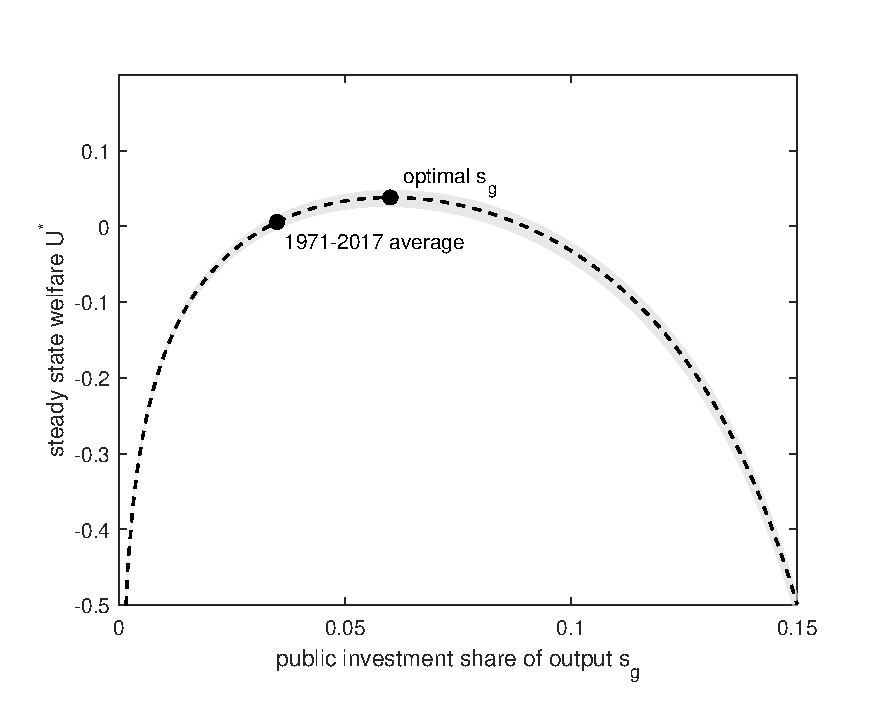
\includegraphics[width=0.8\textwidth]{Laffer_curve_figure_final.pdf}
    \caption{Optimal steady-state public investment share in output}
    \label{fig:laffer_curves}
\end{figure}

Moving from the historical average public investment share of 3.5 per cent to the welfare-optimising level outlined above implies an increase in public investment of approximately 2.5 per cent of output. This corresponds to an almost two thirds increase in the public capital stock. Due to the form of the production function, higher public capital also increases the marginal product of private capital, thereby also raising private investment and capital.
In our framework, any increases in public capital are funded via lower public consumption and crowding out of private consumption, rather than through higher taxation. In the long run, this generates a sizeable increase in output per hour worked, of between 12.2 and 13.1 per cent. These estimates should be interpreted as a reasonable upper bound. 
In practice, it is unlikely that the government could reduce current consumption sufficiently to deliver such a large increase in public investment nor that the entirety of the public capital increase would be efficient and productive. Nevertheless, the results indicate scope for gains from higher public investment as the United Kingdom appears to remain below its welfare-optimal level at the peak of the curve in Figure (\ref{fig:laffer_curves}). Naturally, given the shape of the curve, these gains would become increasingly marginal as we approach our estimated optimal level.



Furthermore, as a final robustness check, we also evaluate the welfare-optimising share of public investment against the condition for dynamic efficiency. This benchmark is informative as it represents the point at which the marginal product of public capital equals its user cost. Beyond this point, the cost of an extra unit of public capital exceeds its marginal product, making further investment sub-optimal - independent of how it is financed. 
The expression $ s_g^*=\frac{\delta_g\theta\beta}{1-\beta+\beta\delta_g}$ implies a ceiling for dynamic efficiency. Using the calibrated and posterior parameter values, we find this gives a share of public investment between 6.6 and 6.8 per cent of output. As expected, this sits above the welfare-optimising level in our model, as public capital is financed through distortionary taxes. This 0.7 percentage point gap between the welfare-optimising level and the dynamic efficient level represents the difference in cost between distortionary funding and lump-sum funding of public investment.


\section{Conclusions} \label{conclusion}
This paper has examined the link between public investment and output in the United Kingdom. Our results firstly provide a UK-specific estimate for the output elasticity of public captial. We estimate a posterior mean of 0.112 for the elasticity, with a tight confidence interval around that estimate. This suggests that public capital has a positive and economically meaningful effect on output in the United Kingdom. 

In our comparative statics analysis, we find that the welfare-maximising public investment to GDP ratio lies between 5.9 and 6.1 per cent of output, above the observed UK average of 3.5 per cent. 
This finding, though interpretable as a reasonable upper bound, suggests that the United Kingdom has scope to benefit from an increase in productive public investment.

Our results hinge on the estimated output elasticity of public capital, a parameter that is known to be challenging to identify empirically. Our conclusions are conditional on our estimation of this parameter, which displays weak local separability from other model parameters. Further progress in quantifying the UK public investment multiplier may require additional data or alternative sources of identification that can improve confidence in our estimates of this parameter.  
We leave this for future work.


\bibliographystyle{agsm} 
\bibliography{TPI_bib2} 

\begin{appendices}
\section{Model derivation} \label{model_derivation_appendix}
\subsection{Households}
The representative household seeks to maximise utility over private consumption, government consumption and leisure, subject to a budget constraint and a private capital accumulation constraint.  At time $t$, the household chooses private consumption $C_t \geq0$, labour supply $N_t$, private investment $I_{p,t}$, next period's private capital $K_{p,t+1} \geq 0$, and this period's private capital utilisation rate $U_{k,t}$.  The household optimisation problem is given by: 

\begin{gather}
    \max\limits_{C_t, N_t, I_{p,t}, K_{p,t+1}, U_{k,t}} \quad \sum_{t=0}^\infty \beta^tU_t \quad \text{s.t} \\
    U_t = \gamma \log(C_t)+ (1-\gamma)\log(G_{c,t}) - \nu \frac{N_t^{1+\eta}}{1+\eta}
    \label{eq:utility_def} \\
    C_t(1+\tau_c) + I_{p,t} = W_tN_t(1-\tau_{n}) + R_{k,t}(1-\tau_k)U_{k,t}K_{p,t} + D_t - T_t \\
    K_{p,t+1} = (1-\underbrace{\delta_{p}U_{k,t}^\phi}_{=\delta_{p,t}})K_{p,t} + I_{p,t}\Big(1-\frac{\kappa}{2}\Big[ \frac{I_{p,t}}{I_{p,t-1}} -1 \Big]^2\Big)X_t
\end{gather}
where $\beta$ is the household subjective discount factor, $\gamma$ is the private consumption utility weight, $\nu$ is the disutility weight on labour; $\eta$ is the inverse Frisch elasticity of labour supply, $\tau_i,  i\in \{c,k,n\}$ represent taxes on consumption, private capital income and labour income; $R_{k,t}$ is the real return to private capital; $W_t$ denotes the real wage; $D_t$ are firm dividends paid to households; $T_t$ denotes a lump-sum government transfer/tax; $\delta_p$ is the private capital depreciation rate; $\delta_{p,t}$ is the private capital effective depreciation rate; $\phi$ governs the magnitude of the effect of increased capital utilisation on the effective depreciation rate; $\kappa$ governs the size of the private investment adjustment cost; and $X_t$ is an exogenous private investment shock. \par 

There are two important frictions on private capital embedded in these equations. Firstly, there is an investment adjustment cost (the size of which is determined by $\kappa$). This friction captures market imperfections and financial constraints which may prevent investment from jumping to its socially optimal level following a shock. We also model variable capacity utilisation of the private capital stock, meaning that the existing stock of private capital can be worked more intensively (via an increase in $U_{k,t}$), but at the cost of accelerated depreciation, where $\phi$ governs the magnitude of that cost. Here, $\delta_p$ represents the baseline rate of physical depreciation and $\delta_{pt} = \delta_{p}U_{k,t}^\phi$ is the effective depreciation rate. When capital is utilised more intensively, the existing stock depreciates more quickly as $\phi > 0$. The product $U_{k,t}K_{p,t} = \tilde{K_{p,t}}$ represents the flow of private capital services. This means that private capital services can adjust immediately in response to a shock, without the firm having to wait one period for investment to roll over into capital stock. Subsequently, it is private capital services which enters as a factor of production.\par

The household first order conditions yield the following optimality conditions: 
a labour-leisure condition;
\begin{equation} \label{labour-leisure}
   W_t(1-\tau_{n}) = \frac{\nu}{\gamma}(1+\tau_c)C_tN_t^\eta
\end{equation}
an Euler equation for private capital,
\begin{equation}\label{Euler_capital2}
    \frac{C_{t+1}}{\beta C_t} = \mathbb{E}_t \Big \{ \frac{Q_{t+1}}{Q_t} \Big[\frac{R_{k,t+1} (1-\tau_k) U_{k,t+1}}{Q_{t+1} }+ (1-\delta_{p,t+1)} \Big] \Big \}
\end{equation}
where $Q_t$ denotes Tobin's Q (the shadow value of investment) adjusted for the shadow value of wealth; 
the first order condition for private capital utilisation; 
\begin{equation} \label{Foc_uk}
    R_{k,t}(1-\tau_k) = \phi Q_t\delta_p U_{k,t}^{\phi-1}\end{equation}

and an Euler equation for investment:

\begin{multline}
1 = Q_t X_t\left[1 - \frac{\kappa}{2}\left(\frac{I_{p,t}}{I_{p,t-1}} - 1\right)^2 + \kappa\frac{I_{p,t}}{I_{p,t-1}}\left(\frac{I_{p,t}}{I_{p,t-1}} - 1\right)\right] \\
+ \kappa\beta Q_{t+1} \frac{C_t}{C_{t+1}} \left(\frac{I_{p,t+1}}{I_{p,t}}\right)^2\left(\frac{I_{p,t+1}}{I_{p,t}} - 1\right)
\end{multline}


\subsection{Firms} 

\subsubsection{Final goods producer}
We assume that there exists a representative firm which produces a final good by bundling intermediate goods produced by a large continuum of firms. This firm produces the final good via the following Dixit-Stiglitz aggregator:

\begin{equation} \label{final_goods_1}
    Y_t= \Bigg[\int_0^1 Y_{j,t}^{\frac{\epsilon -1}{\epsilon}} dj \Bigg]^{\frac{\epsilon}{\epsilon - 1}}
\end{equation}
where $\epsilon > 1$ represents the elasticity of substitution between goods. Each intermediate goods firm $j$ produces their own variety and has monopolistic power to set their own prices (all other prices are treated as given). As $\epsilon \rightarrow \infty$ good varieties become perfect substitutes, and we return to the case of perfect competition. The representative firm which bundles the final good seeks to maximise profit:

\begin{equation} \label{Final_firm_profit_max}
    \max\limits_{Y_t(j)} P_t\Bigg[\int_0^1 Y_{j,t}^{\frac{\epsilon -1}{\epsilon}} dj \Bigg]^{\frac{\epsilon}{\epsilon - 1}} - \int_0^1 P_t(j)Y_t(j) dj
    \end{equation}

The first-order conditions for this firm imply the demand curves for each intermediate good $j$ as a function of its relative price and aggregate output:

\begin{equation} \label{final_firm_demand}
    Y_t(j) = \Big(\frac{P_t(j)}{P_t}\Big)^{-\epsilon}Y_t 
\end{equation}

Combining  (\ref{Final_firm_profit_max}) and (\ref{final_firm_demand}) yields the aggregate price index. This follows logically as the nominal value of the final good is simply the sum of prices times quantities of all the intermediate goods. Without loss of generality, we can normalise the aggregate price level to 1, such that:

\begin{equation}
    P_t = \Big[\int_0^1 P_t(j)^{1-\epsilon}dj\Big]^{\frac{1}{1-\epsilon}} \label{AggPrice} = 1
\end{equation}

\subsubsection{Intermediate good firms}
There is a continuum of measure one of monopolistically competitive intermediate good firms. The intermediate firm producing good $j$ uses the stock of public capital $K_{g,t}$, private capital services $\tilde{K}_{p,t}$ and labour $N_t$ according to the following production function: 
\begin{equation} \label{prod_fn1} 
    Y_t(j) = A_t K_{g,t}^{\theta}\tilde{K}_{p,t}(j)^{\alpha}N_t(j)^{1-\alpha}
\end{equation}
where $\theta$ governs the elasticity of output to public capital, $\alpha$ governs the elasticity of output to private capital, and the elasticity of output to labour is governed by $1-\alpha$ where the 1 ensures that the production function exhibits constant returns to scale in private factors. $A_t$ denotes an aggregate productivity shock.

The firm seeks to minimise production costs given economy-wide the rental rate of capital and real wage, and subject to its production function: 

\begin{gather*}
    \min\limits_{N_t(j),\tilde{K}_{p,t}(j) } \quad W_tN_t(j) + R_{k,t}\tilde{K}_{p,t}(j) \quad 
    s.t \quad (\ref{prod_fn1})
\end{gather*}

which yields the following expression for relative factor demands: 

\begin{gather}
    \frac{\alpha W_t}{(1-\alpha)R_{k,t}U_{kt}} = \frac{{K}_{p,t}(j)}{N_t(j)}
\end{gather}
where the j-index can be dropped as this relative demand is a function of aggregates. Thus, we can derive the following expression for the marginal cost: 

\begin{gather}
    MC_t = \frac{W_t^{(1-\alpha)}R_{k,t}^{\alpha}}{\alpha^\alpha (1-\alpha)^{(1-\alpha)} A_t K_{g,t}^\theta}
\end{gather}

The intermediate good firm then seeks to maximise profits given their production technology and the demand for their variety $j$: 

\begin{gather*}
    \max\limits_{P_t(j)} \quad Y_t(j)P_t(j) - MC_t Y_t(j) \\
    s.t \quad (\ref{final_firm_demand})
\end{gather*}
which yields the standard result that all intermediate good firms will charge the same price of a markup over the marginal cost.


\subsection{Fiscal policy}


We can assume, without loss of generality, zero net supply of bonds. As such, the government must run a balanced budget each period: 

\begin{equation} \label{gov_BC}
    G_{c,t} + I_{g,t} = \tau_c C_t + \tau_nW_tN_t + \tau_kR_{k,t}\tilde{K}_{p,t}
\end{equation}

Government consumption spending is set to maximise the utility of households. That is, the government will increase its consumption spending up to the point at which the marginal utility to the household of an extra unit of government consumption equals the marginal utility of the unit of private consumption that households would need to lose.  

This implies: 

\begin{equation}\label{GC}
G_{c,t} = C_t\Big(\frac{1-\gamma}{\gamma} \Big)G_t
    \end{equation}
where $G_t$ is a government consumption purchases shock.

We set public investment as a fixed proportion, $s_g$, of GDP: 
\begin{equation}\label{GI}
    I_{g,t} = s_gY_tG^s_{i,t}
\end{equation}
where $G^s_{i,t}$ is an exogenous shock to government investment spending.


Drawing from \cite{Suresh24}, we also assume that public investment purchases face time-to-build lags, delaying the process through which public investment tranforms into a part of the productive public capital stock. Let $\omega_n$ be the fraction of $I_{g,t}$ that becomes effective at time $t+n$. We can write the public capital law of motion as:

\begin{equation}
    \label{public_LOM_2}
    K_{g,t+1} = (1-\delta_g)K_{g,t} + \sum_{n=0}^{10}(1-\delta_g)^n \omega_n I_{g,t-n}
\end{equation}



\subsection{Market clearing}
The aggregate resource constraint is given by: 

\begin{equation}
    Y_t = C_t + I_{p,t} + G_{c,t} + I_{g,t}
\end{equation}

\end{appendices}
\end{document}
